\section{Έλεγχος κινητήρα με σταθερή διαταραχή}
Ο κώδικας του ελέγχου εξαρτάται από τα εξής νέα αρχεία:
\begin{itemize}
\item \texttt{lab3.m}: Βασική συνάρτηση για τον έλεγχο.
  Χρησιμοποιεί και τα αρχεία που αναφέρθηκαν στο προηγούμενο εργαστήριο.

  Για τον υπολογισμό του \mintinline{MATLAB}!z! χρησιμοποιείται η μέθοδος του Euler.
  Αρχικά, αρχικοποιείται στη τιμή $-x_1$:
  \begin{code}
\begin{minted}{MATLAB}
[z, ~] = read_state(a, params.Vref_arduino, params.V_7805);
z = -z;
\end{minted}
  \end{code}
  και η ανανέωση της τιμής γίνεται ως εξής:
  \begin{code}
\begin{minted}{MATLAB}
t = toc;
dt = t - last;
z_dot = x_1 - 5;
dz = z_dot * dt;
z = z + dz;
\end{minted}
  \end{code}

  Για την εύρεση των $a_1$, $a_2$, $a_3$ χρησιμοποιείται η συνάρτηση \mintinline{MATLAB}{find_desired}:
  \begin{code}
\begin{minted}{MATLAB}
function [a_1, a_2, a_3] = find_desired(z, omega)
alpha = [1, 2 * z * omega, omega^2];
poles = roots(alpha);
poles = [poles; 4 * min(poles(1), poles(2))];
alpha = poly(poles);
a_1 = alpha(2);
a_2 = alpha(3);
a_3 = alpha(4);
end
\end{minted}
  \end{code}
  Οι πόλοι $p_1$ και $p_2$ βρίσκονται όπως και πριν και ο $p_3$ επιλέγεται να είναι τετραπλάσιος του μικρότερου
  (μεγαλύτερου σε απόλυτη τιμή αρνητικού).

  \item \texttt{lab31.m}: Βοηθητικό script για τη κλήση της προηγούμενης συνάρτησης.
\end{itemize}

\begin{figure}[htbp]
  \centering
  \begin{subfigure}[t]{\linewidth}
    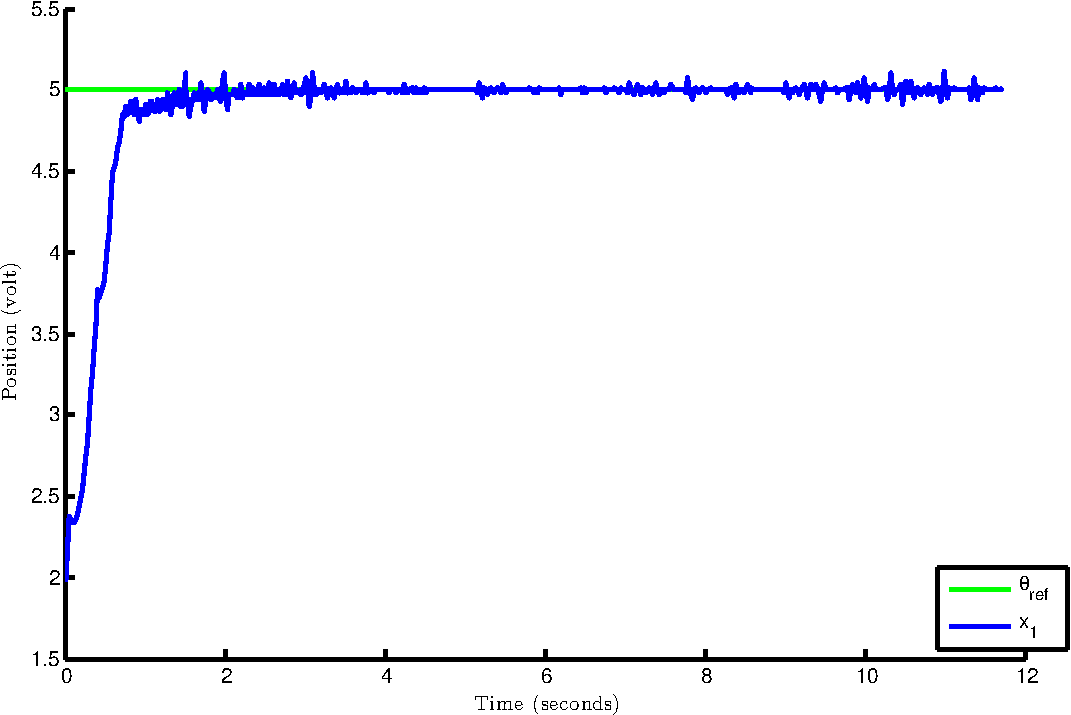
\includegraphics[width=\linewidth, keepaspectratio]{lab3/3-1-x_1}
    \caption{θέση}
    \label{fig:3-1-x_1}
  \end{subfigure}\\
  \begin{subfigure}[t]{0.45\linewidth}
    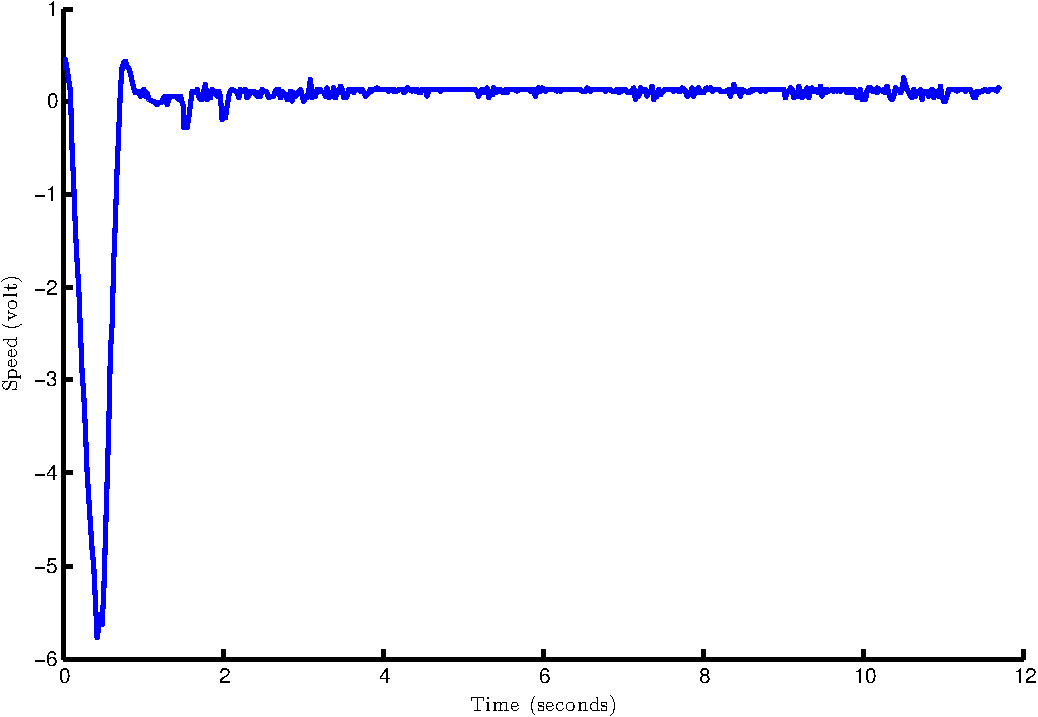
\includegraphics[width=\linewidth, keepaspectratio]{lab3/3-1-x_2}
    \caption{Ταχύτητα}
    \label{fig:3-1-x_2}
  \end{subfigure}\hfill
  \begin{subfigure}[t]{0.45\linewidth}
    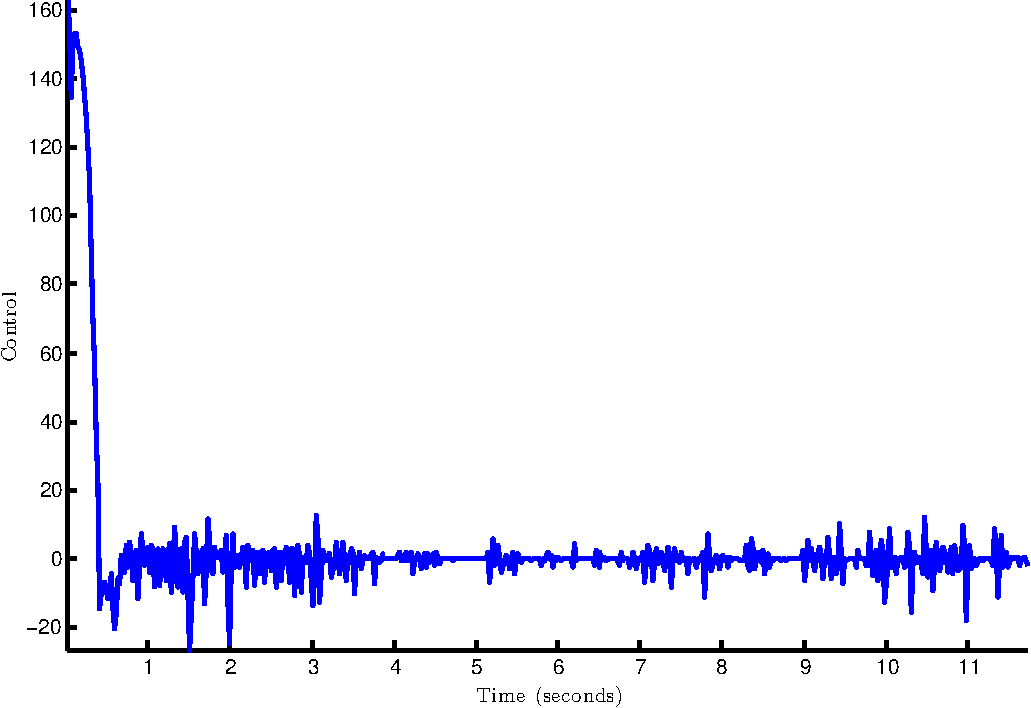
\includegraphics[width=\linewidth, keepaspectratio]{lab3/3-1-u}
    \caption{Είσοδος ελέγχου}
    \label{fig:3-1-u}
  \end{subfigure}
  \caption[]{}
  \label{fig:3-1}
\end{figure}

Αρχικά, δοκιμάζουμε τον έλεγχο χωρίς διαταραχές.
Τα σχετικά διαγράμματα φαίνονται στο σχήμα~\ref{fig:3-1} και τα δεδομένα από τη \texttt{stepinfo} είναι:
\begin{code}
\begin{minted}{text}
    RiseTime: 0.6336
SettlingTime: 11.3764
  SettlingMin: 4.7507
  SettlingMax: 5.1173
    Overshoot: 2.3460
  Undershoot: 0
        Peak: 5.1173
    PeakTime: 10.9843
\end{minted}
\end{code}
Παρατηρούμε ότι υπάρχει μια μικρο-ταλάντωση στη σταθερή κατάσταση.
Αυτό πρέπει να οφείλεται στην ανακρίβεια των μετρήσεων που μπορεί να οδηγήσει και σε λανθασμένη κίνηση του κινητήρα.

\begin{figure}[htbp]
  \centering
  \begin{subfigure}[t]{\linewidth}
    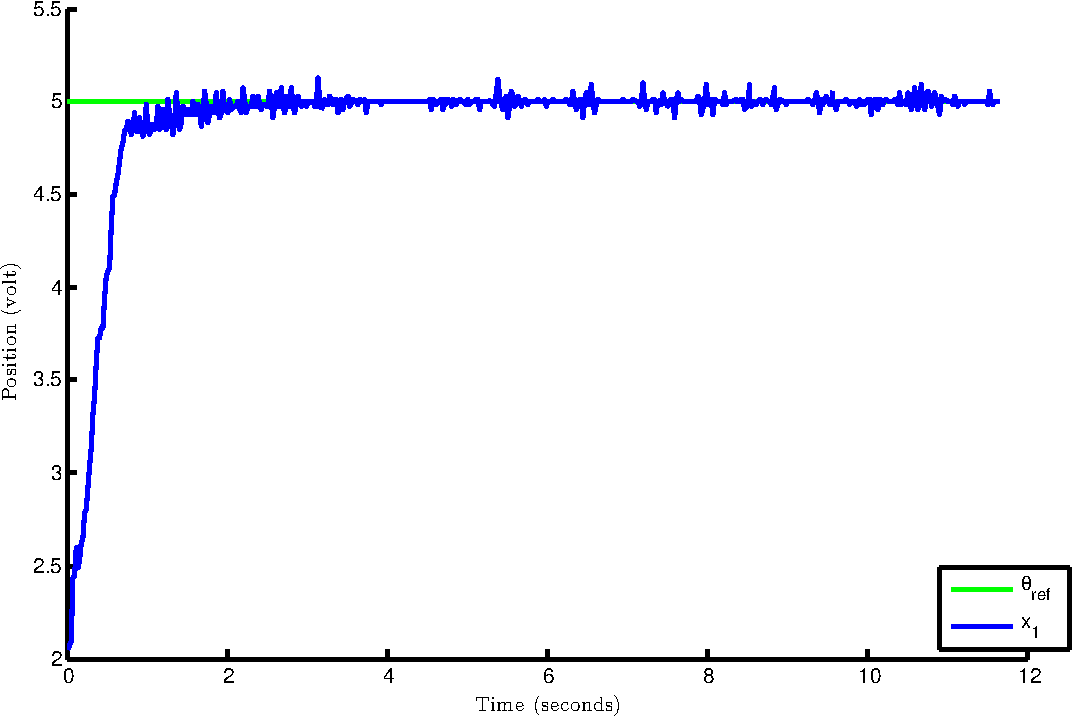
\includegraphics[width=\linewidth, keepaspectratio]{lab3/3-2-x_1}
    \caption{θέση}
    \label{fig:3-2-x_1}
  \end{subfigure}\\
  \begin{subfigure}[t]{0.45\linewidth}
    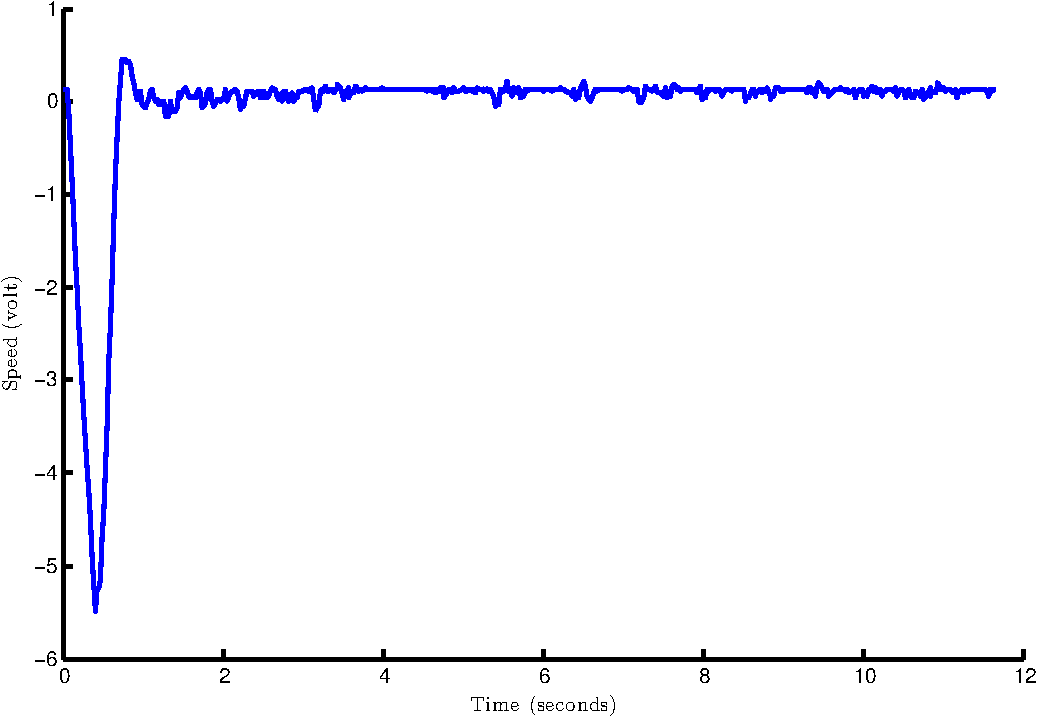
\includegraphics[width=\linewidth, keepaspectratio]{lab3/3-2-x_2}
    \caption{Ταχύτητα}
    \label{fig:3-2-x_2}
  \end{subfigure}\hfill
  \begin{subfigure}[t]{0.45\linewidth}
    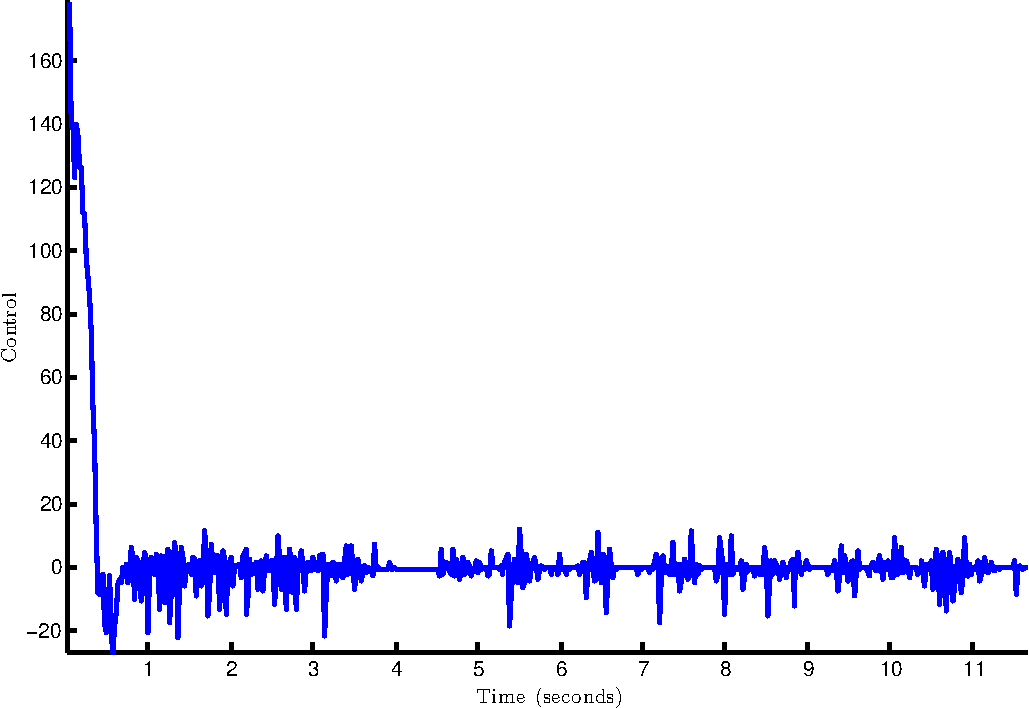
\includegraphics[width=\linewidth, keepaspectratio]{lab3/3-2-u}
    \caption{Είσοδος ελέγχου}
    \label{fig:3-2-u}
  \end{subfigure}
  \caption[]{}
  \label{fig:3-2}
\end{figure}

Στη συνέχεια, δοκιμάζουμε να κατεβάσουμε το μαγνητικό φρένο που προσφέρει μια σταθερή διαταραχή στο σύστημα.
Τα σχετικά διαγράμματα φαίνονται στο σχήμα~\ref{fig:3-2} και τα δεδομένα από τη \texttt{stepinfo} είναι:
\begin{code}
\begin{minted}{text}
    RiseTime: 0.5971
SettlingTime: 10.9036
  SettlingMin: 4.7507
  SettlingMax: 5.1320
    Overshoot: 2.6393
  Undershoot: 0
        Peak: 5.1320
    PeakTime: 3.1337
\end{minted}
\end{code}
Παρατηρούμε ότι το σύστημα δουλεύει όπως επιθυμούμε και σταθεροποιείται στη θέση $\theta_{ref} = \SI{5}{\volt}$ παρά τις διαταραχές.

\begin{figure}[htbp]
  \centering
  \begin{subfigure}[t]{\linewidth}
    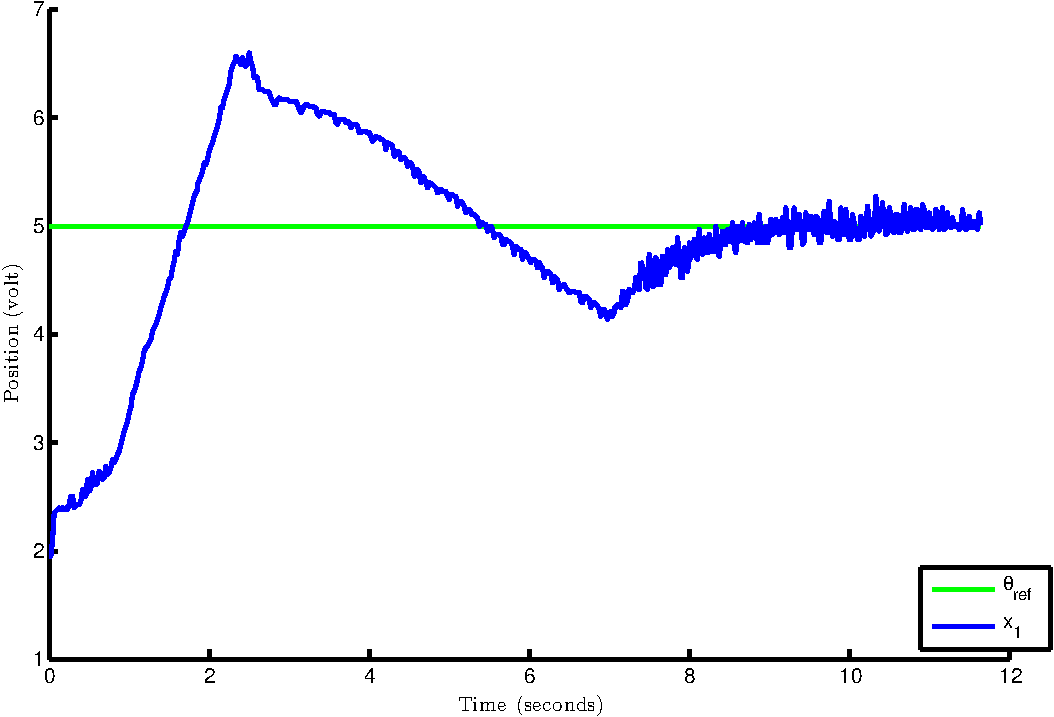
\includegraphics[width=\linewidth, keepaspectratio]{lab3/3-3-x_1}
    \caption{θέση}
    \label{fig:3-3-x_1}
  \end{subfigure}\\
  \begin{subfigure}[t]{0.45\linewidth}
    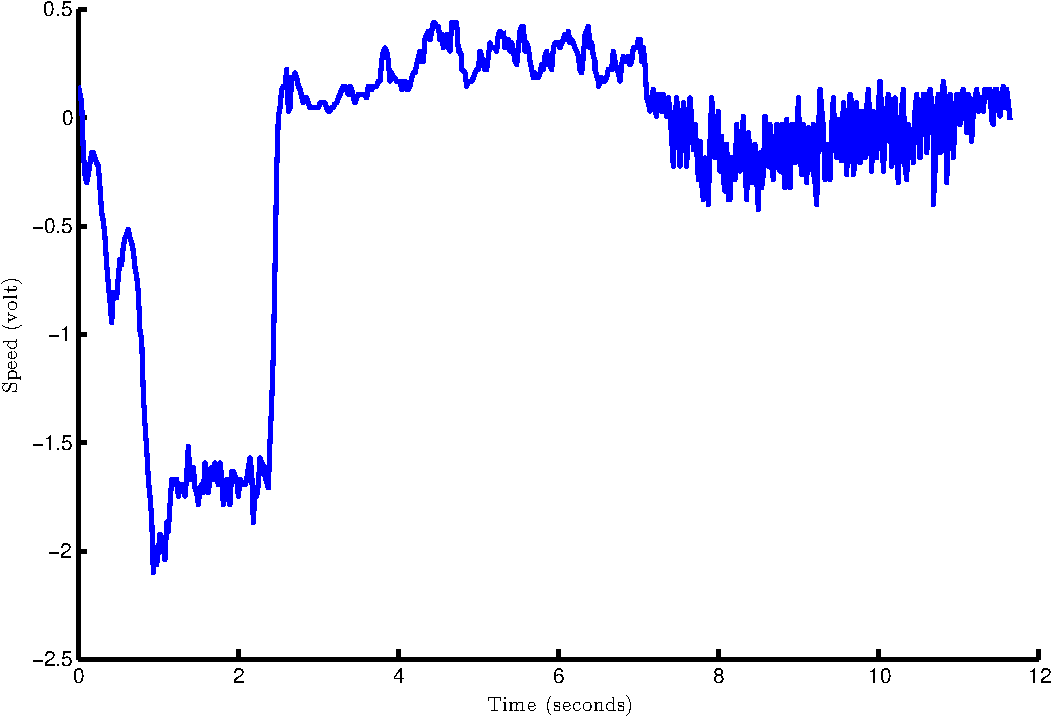
\includegraphics[width=\linewidth, keepaspectratio]{lab3/3-3-x_2}
    \caption{Ταχύτητα}
    \label{fig:3-3-x_2}
  \end{subfigure}\hfill
  \begin{subfigure}[t]{0.45\linewidth}
    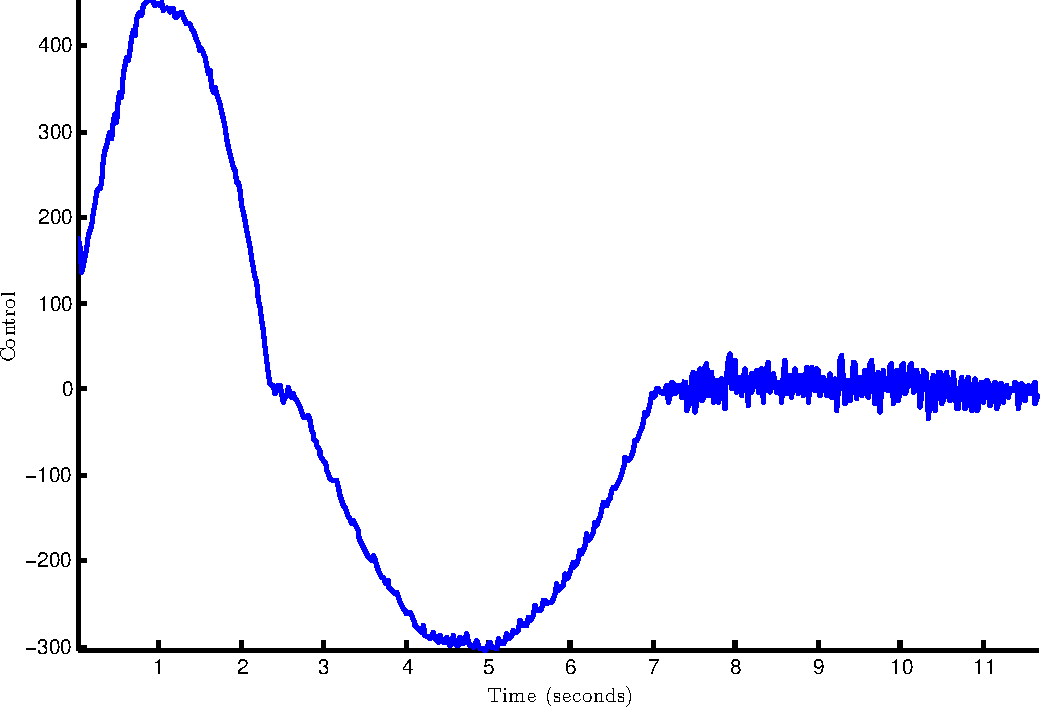
\includegraphics[width=\linewidth, keepaspectratio]{lab3/3-3-u}
    \caption{Είσοδος ελέγχου}
    \label{fig:3-3-u}
  \end{subfigure}
  \caption[]{}
  \label{fig:3-3}
\end{figure}

Τελικά, δοκιμάζουμε να προσφέρουμε διαταραχές πιάνοντας το δισκόφρενο όσο ο κινητήρας δουλεύει.
Τα σχετικά διαγράμματα φαίνονται στο σχήμα~\ref{fig:3-3} και τα δεδομένα από τη \texttt{stepinfo} είναι:
\begin{code}
\begin{minted}{text}
    RiseTime: 1.5163
SettlingTime: 11.6515
  SettlingMin: 4.1349
  SettlingMax: 6.5982
    Overshoot: 31.9648
  Undershoot: 0
        Peak: 6.5982
    PeakTime: 2.5043
\end{minted}
\end{code}
Παρατηρούμε σημαντικό overshoot. Αυτό μπορεί να οφείλεται στο ότι οι διαταραχές δεν είναι σταθερές και στο ότι εισάγεται μια
αρκετά μεγαλύτερη δύναμη στο σύστημα.
%%% Local Variables:
%%% mode: latex
%%% TeX-master: "../lab3"
%%% End:
